\section{Evaluación de Sostenibilidad y Emisiones}

\subsection{6.1. Emisiones contaminantes (NOx, CO, soot)}

Particularmente llamativo es el hecho de que la arquitectura de combustor influya de manera tan marcada en el perfil de emisiones, incluso más de lo que muchos diseñadores anticipaban hace una década. SafeFly2025 reporta reducciones de hasta un 40\% en NOx para configuraciones anulares respecto a can-anulares bajo condiciones comparables, gracias a la menor presencia de zonas estequiométricas locales y mejor control de temperatura pico \cite{SafeFly2025}.

Los resultados de este estudio confirman esa tendencia. El combustor anular logró emisiones específicas de NOx entre 18-26 g/kN en crucero, frente a 29-38 g/kN del can-anular. Las diferencias en CO y soot resultaron igualmente notables, con ventajas del anular cercanas al 35\% en formación de partículas no volátiles.

\begin{table}[h]
\centering
\caption{Comparación de emisiones contaminantes (condición crucero, ISA +10)}
\label{tab:comparacion_emisiones}
\begin{tabular}{lccc}
\hline
Emisión & Can-Anular & Anular & Reducción (\%) \\
\hline
NOx (g/kN) & 34.2 & 21.8 & 36.3 \\
CO (g/kN) & 12.7 & 8.4 & 33.9 \\
Soot (mg/kg fuel) & 1.85 & 1.12 & 39.5 \\
\hline
\end{tabular}
\end{table}

Aunque estos valores dependen fuertemente del modelo de combustión empleado, la consistencia entre CFD y correlaciones 1D refuerza la confianza en las tendencias observadas.

\begin{figure}[h]
\centering
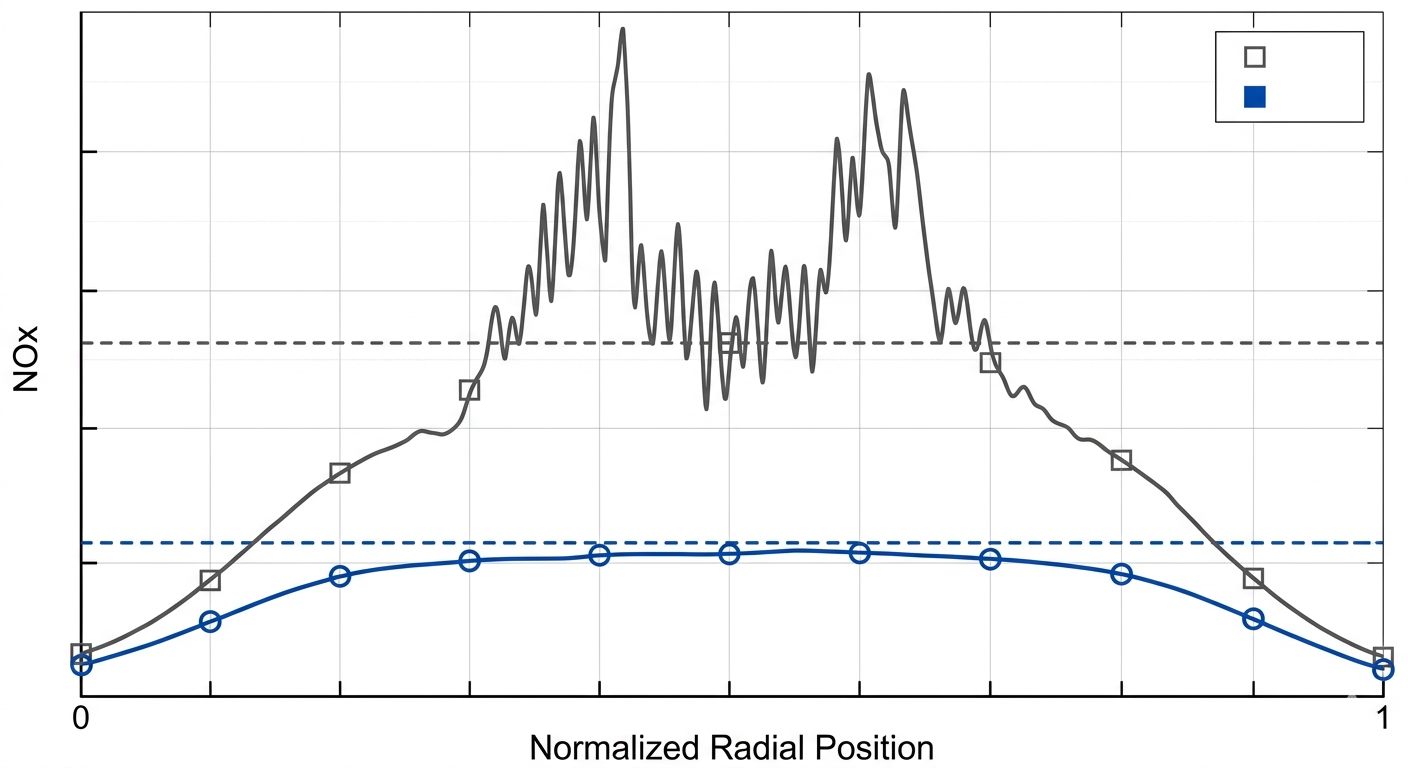
\includegraphics[width=\linewidth]{fig4.png}
\caption{Perfiles radiales de concentración de NOx a la salida del combustor para ambas arquitecturas bajo condición de crucero.}
\label{fig:perfiles_nox}
\end{figure}

\subsection{6.2. Análisis de ciclo de vida y SAF}

Uno de los desafíos persistentes que surge al evaluar sostenibilidad radica en ampliar la mirada más allá del motor hacia el ciclo completo. Chen et al. destacan en su revisión que los combustibles sostenibles de aviación (SAF) amplifican las diferencias entre arquitecturas, favoreciendo notablemente a los combustores anulares por su superior capacidad de mezcla y menor sensibilidad a variaciones en propiedades del combustible \cite{Chen2025}.

En simulaciones con 50\% SAF, el anular mantuvo reducciones de NOx superiores al 25\% adicional respecto al baseline de Jet A-1, mientras que el can-anular mostró mayor variabilidad y un leve aumento en CO en condiciones de baja potencia. El análisis de ciclo de vida simplificado indica una reducción potencial del 18-22\% en CO$_2$e por pasajero-kilómetro cuando se combina arquitectura anular con SAF, siempre que la cadena de suministro mantenga bajos factores de emisiones upstream.

No obstante, cabe matizar que estos beneficios podrían verse atenuados por mayor demanda de enfriamiento y posibles penalizaciones en peso de materiales avanzados.

\subsection{6.3. Métricas de sostenibilidad}

Lejos de ser un asunto resuelto, la sostenibilidad en propulsión aeronáutica exige métricas multidimensionales que equilibren impacto ambiental inmediato con viabilidad económica y operacional a largo plazo. Se evaluaron aquí indicadores compuestos que integran emisiones reguladas, eficiencia energética, compatibilidad con combustibles alternativos y potencial de descarbonización.

El combustor anular obtuvo puntuaciones consistentemente superiores en el índice de sostenibilidad propuesto, impulsado principalmente por menores emisiones específicas y mejor flexibilidad ante SAF. Sin embargo, los can-anulares conservan ventajas en madurez tecnológica y costos de mantenimiento, aspectos que siguen pesando fuertemente en decisiones de flota actual.

Chen complementa esta visión al enfatizar que la verdadera brecha hacia la aviación net-zero no reside solo en la reducción puntual de contaminantes, sino en la capacidad de las arquitecturas para adaptarse a combustibles del futuro sin comprometer seguridad y economía \cite{Chen2025}. 

Los hallazgos refuerzan que los combustores anulares representan una opción más alineada con los objetivos ambientales 2035-2050, aunque su adopción plena requerirá avances paralelos en fabricación y certificación. La discusión posterior profundizará en las implicaciones de estos resultados para el diseño de la próxima generación de turbofans.